% Shared preamble for the CIG-AMF formal-research papers.
% IEEEtran conference class; compiles on Overleaf without modification.
\documentclass[conference]{IEEEtran}
\IEEEoverridecommandlockouts

\usepackage{cite}
\usepackage{amsmath,amssymb,amsfonts}
\usepackage{amsthm}
\usepackage{algorithm}
\usepackage{algorithmic}
\usepackage{graphicx}
\usepackage{textcomp}
\usepackage{xcolor}
\usepackage{booktabs}
\usepackage{url}
\usepackage[hidelinks]{hyperref}

\def\BibTeX{{\rm B\kern-.05em{\sc i\kern-.025em b}\kern-.08em T\kern-.1667em\lower.7ex\hbox{E}\kern-.125emX}}

\newtheorem{theorem}{Theorem}
\newtheorem{lemma}[theorem]{Lemma}
\newtheorem{proposition}[theorem]{Proposition}
\newtheorem{corollary}[theorem]{Corollary}
\theoremstyle{definition}
\newtheorem{definition}[theorem]{Definition}
\newtheorem{remark}[theorem]{Remark}
\newtheorem{example}[theorem]{Example}

% A machine-checked statement carries its Lean declaration name.
\newcommand{\lean}[1]{\textsf{\footnotesize #1}}
\newcommand{\leanbox}[1]{%
  \par\vspace{2pt}\noindent
  {\footnotesize\textsf{Lean: #1}}\par\vspace{2pt}}

% Evidence classes, used consistently and never interchangeably.
\newcommand{\PROVED}{\textsc{proved}}
\newcommand{\CERT}{\textsc{certificate}}
\newcommand{\NUM}{\textsc{numerical}}
\graphicspath{{../_figures/}}


\begin{document}

\title{The Slice Is Not a Restriction,\\
and the Design Is Not Fitted}

\author{\IEEEauthorblockN{Vu Phan An Nguyen}
\IEEEauthorblockA{\textit{Rider University} \\
Lawrenceville, NJ, USA}}

\maketitle

\begin{abstract}
A scalar query measures $q$ coordinates and must distinguish the truth from an alternative.
Its per-sample information is customarily stated against an alternative parameterised by
$(d,x)$: $d$ coordinates displaced by $\mu$, the remaining $q-d$ displaced by $x$. Two
objections stand against using that statement. A bound proved only over a two-parameter
\emph{slice} says nothing about alternatives outside it, so a lower bound quantified over
$(d,x)$ is not a lower bound over the class; and the design weights reproducing the
coefficients were \emph{fitted}---a consistent non-negative solution in $24$ of $24$
parameter cells is evidence, not a derivation. Neither objection is answered by more cells
or more search; each needs an argument, and this paper supplies both. We define the general
alternative as an arbitrary shift vector, show the $(d,x)$ formula is exactly the general
information evaluated on the slice, and prove that \emph{every} alternative in the class
costs at least the slice value, with equality precisely on the slice---so the reduction
loses nothing and gains nothing. The same computation shows the general information vanishes
only at the zero shift, so the scalar query is blind in no direction whatsoever. We then
prove that the budget constraint together with the split \emph{forces} the two weights,
which therefore depend on the split $\eta$ and the price $c$ alone and not on the model
parameters $(q,\mu)$; the delivered information is consequently affine in the split, so the
optimum sits at an endpoint unless the two queries buy information at exactly the same rate
per unit price---a condition we derive and on which every split is optimal. Each displayed theorem is machine-checked in Lean~4 with no \texttt{sorry}; the corollaries the paper derives from them are marked in Section~\ref{sec:verification}.
\end{abstract}

\begin{IEEEkeywords}
experimental design, information bounds, alternative families, budget allocation,
formal verification, interactive theorem proving
\end{IEEEkeywords}

\section{Introduction}

A scalar query measures $q$ coordinates at once and returns a noisy scalar summary. To
certify an answer it must distinguish the truth from an alternative, and the standard way to
state what it can do is to fix a two-parameter family of alternatives---$d$ coordinates
displaced by $\mu$, the remaining $q-d$ displaced by $x$---and compute the per-sample
information $I_{B}(d,x)$ against that family.

This is convenient and it is what a corpus of results is stated against. It is also open to
two objections that no amount of further computation answers.

\subsection{The two objections}

\emph{The slice objection.} A lower bound proved by quantifying over $(d,x)$ is a lower
bound over a two-dimensional slice of a $q$-dimensional alternative class. An alternative
outside the slice---one whose displacements are not constant on two blocks---is not covered,
and for all the bound says it could be cheaper. A slice-quantified lower bound is therefore
not a class-quantified one, and using it as though it were is a quantifier error.

\emph{The provenance objection.} The design weights that reproduce the corpus's coefficients
were obtained by fitting. A consistent non-negative solution in $24$ of $24$ parameter cells
is good evidence that the coefficients come from the model rather than from the fit; it is
not a derivation, and the difference matters if the weights are to be used outside the cells
tested.

Neither objection is answered by more cells or more search. Each needs an argument, and
Sections~\ref{sec:reduction} and \ref{sec:design} supply them.

\subsection{Why these are the right objections to answer}

Both objections are about the \emph{status} of a result rather than its value, and that is
what makes them worth a paper. Neither says the corpus's bounds are numerically wrong. The
slice objection says a true statement about a slice has been used as though it were a true
statement about a class; the provenance objection says a formula that fits is being used as
though it were a formula that follows. In each case the arithmetic is unchanged by the
repair, and what changes is what may be concluded from it.

This also fixes what would count as an answer. For the slice objection, an answer must be a
universally quantified theorem, because no finite collection of alternatives sampled from
outside the slice can establish a claim about all of them. For the provenance objection, an
answer must be a derivation from the constraints, because a fit that succeeds in more cells
is still a fit. Sections~\ref{sec:reduction} and \ref{sec:design} are constructed to meet
exactly these bars and nothing looser.

\subsection{Contributions}

\begin{enumerate}
\item[C1.] \textbf{The slice is not a restriction.} We define the general alternative as an
arbitrary shift vector, show the $(d,x)$ formula is exactly that general information
evaluated on the slice (Theorem~\ref{thm:slice}), and prove that every alternative in the
class costs at least the slice value (Theorem~\ref{thm:reduction}). A lower bound quantified
over the slice is therefore a lower bound over the whole class.

\item[C2.] \textbf{The slice is exactly tight.} The bound of C1 is attained precisely on the
slice (Corollary~\ref{cor:tight}), so it cannot be improved by enlarging the class.

\item[C3.] \textbf{No blind direction at all.} The general information vanishes only at the
zero shift (Theorem~\ref{thm:nonblind}), so the scalar query is blind in no direction
whatsoever.

\item[C4.] \textbf{The design is derived, not fitted.} The budget constraint together with
the split forces the two weights (Theorems~\ref{thm:budget}, \ref{thm:unique}), which depend
on $(\eta,c)$ alone and not on $(q,\mu)$ (Corollary~\ref{cor:indep}).

\item[C5.] \textbf{Where a transition can occur, derived.} The delivered information is
affine in the split (Theorem~\ref{thm:affine}), so the optimum sits at an endpoint unless
$c\,I_{B}=I_{\mathrm{pair}}$, and on that condition every split is optimal
(Theorem~\ref{thm:transition}).
\end{enumerate}

\subsection{Roadmap}

Section~\ref{sec:setting} fixes notation and Section~\ref{sec:related} the novelty boundary.
Section~\ref{sec:reduction} answers the slice objection: the general alternative, the
identity on the slice, the reduction, tightness and non-blindness.
Section~\ref{sec:worked} works a numerical instance and Section~\ref{sec:reading} says what
the upgraded bound does and does not license. Section~\ref{sec:design} answers the
provenance objection by deriving the weights, and derives the affine structure and the
transition condition that follow. Section~\ref{sec:certificate} covers the separation
certificate, Section~\ref{sec:transition} reads the transition condition carefully,
Section~\ref{sec:results} reports the cells, Section~\ref{sec:verification} the formal
development, and Section~\ref{sec:discussion} the scope.

The two halves are independent as arguments and joined as a conclusion: the reduction makes
$I_{B}$ the right quantity to bound, and the design derivation makes it the quantity a
design delivers. Section~\ref{sec:discussion} returns to why neither is complete alone.

\section{Setting and notation}
\label{sec:setting}

\begin{table}[htbp]
\caption{Notation.}
\label{tab:notation}
\centering
\footnotesize
\begin{tabular}{@{}ll@{}}
\toprule
Symbol & Meaning \\
\midrule
$q$ & coordinates measured by the scalar query \\
$v\in\mathbb{R}^{q}$ & a general shift vector (the alternative) \\
$S$ & the displaced block, $|S|=d$ \\
$d$ & size of the displaced block \\
$\mu$ & displacement on $S$ \\
$x$ & displacement off $S$ \\
$I(v)$ & general per-sample information, \eqref{eq:igen} \\
$I_{B}(d,x)$ & slice information, \eqref{eq:ib} \\
$I_{\mathrm{pair}}$ & information of the pair query \\
$c$ & price of the pair query, scalar query $=1$ \\
$\eta$ & budget share committed to the pair query \\
$w_{B},w_{\mathrm{pair}}$ & design weights \\
$I(\eta)$ & delivered information at split $\eta$ \\
$\rho,r$ & modulus propagation factors \\
\bottomrule
\end{tabular}
\end{table}

The \emph{class} of alternatives is cut out by per-coordinate magnitude constraints: a shift
$v$ belongs to the class determined by $(S,\mu,x)$ when $|v_{i}|\ge\mu$ for $i\in S$ and
$|v_{i}|\ge x$ for $i\notin S$, with $|S|=d$. The slice is the sub-family in which every
inequality holds with equality and every sign is the same.

\section{Related work and the novelty boundary}
\label{sec:related}

\subsection{Alternative families in design and testing}

Reducing a high-dimensional alternative class to a low-dimensional family is an old device.
In optimal design it appears as the restriction of the criterion to a parametric direction
\cite{pukelsheim2006,fedorov1972}; in testing it appears as the choice of a least-favourable
alternative. The device is sound when the restriction is shown to be extremal, and unsound
when it is merely convenient, and the distinction is not always drawn: a family chosen for
computability may or may not contain the minimiser.

The present paper draws it explicitly for one case. Theorem~\ref{thm:reduction} shows the
$(d,x)$ family is extremal within the magnitude-constrained class, and
Corollary~\ref{cor:tight} that it is exactly so. Neither statement is deep; what is new is
that the status of the family is settled rather than assumed, and settled in the direction
that licenses the existing bounds.

\subsection{Budget-constrained allocation}

Allocating a budget between measurement types under a linear price is a standard convex
programme \cite{boyd2004}, and the affine structure of Theorem~\ref{thm:affine} is a special
case of the observation that a linear objective over a simplex attains its optimum at a
vertex. What is specific here is that the reduction to an affine objective is not assumed
but derived: it follows from Theorem~\ref{thm:unique}, which removes the apparent freedom in
the weights and leaves the split as the only variable.

Without that step one would be optimising over a two-dimensional weight space subject to one
budget constraint, and the objective on that space is linear but the feasible set is a
segment whose parameterisation is not obviously the split. Fixing the parameterisation is
what makes \eqref{eq:transitioncond} readable as ``equal information per unit price'' rather
than as an arbitrary algebraic condition.

\subsection{Interval and rational certificates}

The enclosure discipline of Section~\ref{sec:certificate} is standard interval arithmetic
\cite{moore2009} carried out over the rationals so that the enclosures are exact rather than
outward-rounded floats. Nothing about the technique is new; it is used here because the
conclusions are strict inequalities, and a strict inequality established in floating point
is not established.

\subsection{Summary of the boundary}

The information-matrix apparatus and the notion of an optimal design on a fixed design space
are standard \cite{pukelsheim2006}, as is the convex-analytic treatment of budget-constrained
allocation \cite{boyd2004}. The information formulas $I_{B}$ and $I_{\mathrm{pair}}$ are
taken as given from the corpus and are not re-derived here from the sampling model; the
paper's subject is what can be concluded \emph{from} them, not where they come from.

What is claimed as new is narrow and methodological. C1 and C2 concern a quantifier: they
convert a slice-quantified lower bound into a class-quantified one and show the conversion
is lossless. C4 concerns provenance: it replaces a fit with a derivation. C5 is the
consequence of C4, and it is a statement about where an optimal design can change character.
None of these is a new bound, a new estimator or a new algorithm, and none is claimed as
such.

\section{The general alternative and the reduction}
\label{sec:reduction}

\subsection{Two formulas, one object}

\begin{definition}[General and slice information]
For a shift vector $v\in\mathbb{R}^{q}$,
\begin{equation}
I(v)\;=\;\frac{1}{2q}\sum_{i=1}^{q} v_{i}^{2},
\label{eq:igen}
\end{equation}
and for the two-parameter family,
\begin{equation}
I_{B}(d,x)\;=\;\frac{1}{2}\left(\frac{d\,\mu^{2}}{q}+\frac{(q-d)\,x^{2}}{q}\right).
\label{eq:ib}
\end{equation}
\end{definition}

\begin{theorem}[The slice identity]
\label{thm:slice}
If $v_{i}=\mu$ for $i\in S$ with $|S|=d$ and $v_{i}=x$ for $i\notin S$, then
$I(v)=I_{B}(d,x)$.
\end{theorem}

\begin{proof}
Split the index set into $S$ and its complement. The summand is constant on each part, so
$\sum_{i}v_{i}^{2}=d\mu^{2}+|S^{c}|x^{2}$, and $|S^{c}|=q-d$ by the cardinality identity
for complements. Dividing by $2q$ gives \eqref{eq:ib}.
\end{proof}

\leanbox{\lean{Igen}, \lean{IB\_eq\_of\_slice} in \lean{LeanD6GeneralFamilyV1}}

Theorem~\ref{thm:slice} is stated first because without it the two objections could not even
be posed together: it establishes that \eqref{eq:igen} and \eqref{eq:ib} are not two
different models but one expression written two ways.

\subsection{The reduction}

\begin{theorem}[Every alternative costs at least the slice value]
\label{thm:reduction}
If $|v_{i}|\ge\mu$ for $i\in S$, $|v_{i}|\ge x$ for $i\notin S$, and $|S|=d$, then
\begin{equation}
I_{B}(d,x)\;\leq\;I(v).
\label{eq:reduction}
\end{equation}
\end{theorem}

\begin{proof}
For $i\in S$, monotonicity of the square on non-negative arguments gives
$v_{i}^{2}=|v_{i}|^{2}\ge\mu^{2}$; for $i\notin S$ likewise $v_{i}^{2}\ge x^{2}$. Summing
over $S$ and over its complement,
$\sum_{i}v_{i}^{2}\ge d\mu^{2}+(q-d)x^{2}$, and dividing by the positive normaliser $2q$
gives \eqref{eq:reduction}.
\end{proof}

\leanbox{\lean{IB\_le\_general} in \lean{LeanD6GeneralFamilyV1}}

No optimiser and no rearrangement argument is needed: the bound is coordinate-wise and the
sum is finite. This is worth noting because a reduction of this kind is often attempted by
an exchange argument, which requires care about which coordinate is moved and in what order;
here the monotonicity of the square does all the work.

\begin{corollary}[The slice is exactly tight]
\label{cor:tight}
Equality holds in \eqref{eq:reduction} precisely when $|v_{i}|=\mu$ on $S$ and $|v_{i}|=x$
off it, i.e.\ precisely on the slice.
\end{corollary}

\begin{proof}
Each coordinate inequality in the proof of Theorem~\ref{thm:reduction} is strict unless the
magnitude is at its bound, and a sum of non-negative terms vanishes only when each does.
Conversely Theorem~\ref{thm:slice} gives equality on the slice.
\end{proof}

\leanbox{\lean{slice\_is\_tight} in \lean{LeanD6GeneralFamilyV1}}

\subsection{What C1 and C2 together mean}

Theorem~\ref{thm:reduction} says the slice is the cheapest member of its class;
Corollary~\ref{cor:tight} says it is exactly the cheapest, attained rather than approached.
The pair has a precise consequence for how the corpus's bounds may be used.

\begin{corollary}[Quantifier upgrade]
\label{cor:upgrade}
If $L\le I_{B}(d,x)$ for every $(d,x)$ in the slice, then $L\le I(v)$ for every $v$ in the
class. Conversely no bound better than $\inf_{\text{slice}}I_{B}$ holds over the class.
\end{corollary}

The first half is the upgrade the paper set out to obtain: a lower bound proved over the
two-parameter family is a lower bound over the whole class, so the family stops being a
limitation. The second half is the tightness statement, and it is what makes the upgrade
free rather than lossy---enlarging the class would not have produced a better bound anyway.

\begin{remark}[Direction matters]
Corollary~\ref{cor:upgrade} converts a \emph{lower} bound. An upper bound quantified over
the slice would still say nothing about the class, because Theorem~\ref{thm:reduction} runs
the wrong way for that purpose. Nothing here licenses an upper-bound upgrade and none is
claimed.
\end{remark}

\subsection{No blind direction}

\begin{theorem}[Positivity]
\label{thm:nonblind}
$I(v)>0$ for every $v\neq0$.
\end{theorem}

\begin{proof}
$I(v)$ is a positive multiple of a sum of squares, which vanishes only when every coordinate
does.
\end{proof}

\leanbox{\lean{Igen\_pos\_of\_ne\_zero} in \lean{LeanD6GeneralFamilyV1}}

The scalar query is therefore blind in no direction whatsoever: a single non-zero coordinate
suffices to make it informative. Stated this way the fact needs no reference to the slice,
and it restates the asymmetry against the pair query---which \emph{does} have a blind
direction---at the level of the general alternative rather than of a two-parameter family.

\section{Reading the reduction as a design statement}
\label{sec:reading}

Sections~\ref{sec:reduction} and \ref{sec:worked} are about a bound. Before turning to the
design it is worth spelling out what the bound does and does not license, because the two
halves of the paper are used together and the join is where a reader could over-claim.

\subsection{What a class-quantified lower bound buys}

A lower bound on the per-sample information against every alternative in the class converts,
in the usual way, into an upper bound on the number of samples needed to exclude the class.
That conversion is not carried out here---it belongs to whatever stopping rule the corpus
uses---but it is the reason the quantifier matters. A stopping rule justified by a
slice-quantified bound is justified against slice alternatives only, and an adversary
choosing an alternative outside the slice is not covered by it.

After Theorem~\ref{thm:reduction} the adversary gains nothing by leaving the slice. This is
the operational content of C1: not that the bound improves, but that the set of adversaries
it covers widens to the whole class at no cost in the constant.

\subsection{What it does not buy}

It does not say that the class is the right class. The magnitude constraints defining it are
a modelling choice, and an alternative that violates them---one that leaves some coordinate
undisplaced, say---is outside every statement here. Nor does it say anything about the pair
query, whose blind direction means that a coordinate-wise argument of the kind used in
Theorem~\ref{thm:reduction} cannot get started: there are non-zero shifts the pair query
cannot see at all, so no positive lower bound holds uniformly over its class.

That asymmetry between the two queries is, in this development, the whole reason a mixed
design is interesting. If both queries were blind in no direction, the choice between them
would be a matter of price alone; because one of them has a kernel and the other does not,
the mixture question has content, and Section~\ref{sec:design} answers what the price does
with it.

\section{The design from its price}
\label{sec:design}

\subsection{The budget forces the weights}

\begin{theorem}[Budget identity]
\label{thm:budget}
With
\begin{equation}
w_{B}=1-\eta,\qquad
w_{\mathrm{pair}}=\frac{\eta}{c},
\label{eq:design}
\end{equation}
the unit budget holds exactly:
\begin{equation}
w_{B}+c\,w_{\mathrm{pair}}\;=\;1 .
\label{eq:budget}
\end{equation}
\end{theorem}

\begin{proof}
$w_{B}+c\,w_{\mathrm{pair}}=(1-\eta)+c\cdot\eta/c=(1-\eta)+\eta=1$. The computation is
rational algebra valid for every split and every positive price.
\end{proof}

\leanbox{\lean{budget\_exact} in \lean{LeanD6DesignDerivationV1}}

\begin{theorem}[Uniqueness]
\label{thm:unique}
Given the split $\eta$---the budget share committed to the pair query---and the price $c>0$,
the pair $(w_{B},w_{\mathrm{pair}})$ satisfying \eqref{eq:budget} is unique and equals
\eqref{eq:design}.
\end{theorem}

\begin{proof}
The budget \eqref{eq:budget} is one linear equation in two unknowns; the split supplies the
second, $c\,w_{\mathrm{pair}}=\eta$. Two independent linear equations in two unknowns
determine the pair.
\end{proof}

\leanbox{\lean{weights\_unique} in \lean{LeanD6DesignDerivationV1}}

\begin{proposition}[Admissible range, derived]
\label{prop:nonneg}
Both weights are non-negative exactly when $0\le\eta\le1$ and $c>0$.
\end{proposition}

\leanbox{\lean{weights\_nonneg\_iff} in \lean{LeanD6DesignDerivationV1}}

The range of the split is therefore derived rather than assumed. This is a small point that
does real work: an implementation that clamps $\eta$ to $[0,1]$ by fiat cannot distinguish a
genuinely infeasible configuration from one it has silently repaired, whereas
Proposition~\ref{prop:nonneg} makes the admissible range a consequence of non-negativity.

\begin{corollary}[Independence of the model parameters]
\label{cor:indep}
$w_{B}$ and $w_{\mathrm{pair}}$ depend on $(\eta,c)$ alone, and not on $(q,\mu)$.
\end{corollary}

\begin{proof}
Neither $q$ nor $\mu$ appears in \eqref{eq:design}, and by Theorem~\ref{thm:unique} no other
solution exists.
\end{proof}

Corollary~\ref{cor:indep} is what answers the provenance objection. The fitted weights were
observed to be constant across $(q,\mu)$ in the cells tested; the derivation explains why,
and extends the statement to every $(q,\mu)$ rather than to the cells.

\begin{table*}[t]
\caption{All 24 parameter cells. The two weight columns are the derived formula
\eqref{eq:design}; they were previously obtained by fitting, and they agree in every cell.
The last column is $w_{B}+c\,w_{\mathrm{pair}}$, exactly $1$ throughout---
Theorem~\ref{thm:budget}. Reading down the table, the weights are constant across $q$ and
$\mu$ and vary only with $(\eta,c)$, which is Corollary~\ref{cor:indep}: the design does not
depend on the model parameters at all.}
\label{tab:cells}
\centering
\footnotesize
\setlength{\tabcolsep}{4pt}
\begin{tabular}{@{}rrrrrrr@{\hspace{10pt}}|@{\hspace{10pt}}rrrrrrr@{}}
\toprule
$q$ & $\mu$ & $c$ & $\eta$ & $w_{B}$ & $w_{\mathrm{pair}}$ & budget & $q$ & $\mu$ & $c$ & $\eta$ & $w_{B}$ & $w_{\mathrm{pair}}$ & budget \\
\midrule
8 & $\frac{1}{4}$ & $\frac{3}{2}$ & $\frac{1}{3}$ & $\frac{2}{3}$ & $\frac{2}{9}$ & $1$ & 16 & $\frac{1}{4}$ & $\frac{3}{2}$ & $\frac{1}{3}$ & $\frac{2}{3}$ & $\frac{2}{9}$ & $1$ \\
8 & $\frac{1}{4}$ & $\frac{3}{2}$ & $\frac{13}{20}$ & $\frac{7}{20}$ & $\frac{13}{30}$ & $1$ & 16 & $\frac{1}{4}$ & $\frac{3}{2}$ & $\frac{13}{20}$ & $\frac{7}{20}$ & $\frac{13}{30}$ & $1$ \\
8 & $\frac{1}{4}$ & $\frac{3}{2}$ & $\frac{4}{5}$ & $\frac{1}{5}$ & $\frac{8}{15}$ & $1$ & 16 & $\frac{1}{4}$ & $\frac{3}{2}$ & $\frac{4}{5}$ & $\frac{1}{5}$ & $\frac{8}{15}$ & $1$ \\
8 & $\frac{1}{4}$ & $2$ & $\frac{1}{3}$ & $\frac{2}{3}$ & $\frac{1}{6}$ & $1$ & 16 & $\frac{1}{4}$ & $2$ & $\frac{1}{3}$ & $\frac{2}{3}$ & $\frac{1}{6}$ & $1$ \\
8 & $\frac{1}{4}$ & $2$ & $\frac{13}{20}$ & $\frac{7}{20}$ & $\frac{13}{40}$ & $1$ & 16 & $\frac{1}{4}$ & $2$ & $\frac{13}{20}$ & $\frac{7}{20}$ & $\frac{13}{40}$ & $1$ \\
8 & $\frac{1}{4}$ & $2$ & $\frac{4}{5}$ & $\frac{1}{5}$ & $\frac{2}{5}$ & $1$ & 16 & $\frac{1}{4}$ & $2$ & $\frac{4}{5}$ & $\frac{1}{5}$ & $\frac{2}{5}$ & $1$ \\
8 & $\frac{2}{5}$ & $\frac{3}{2}$ & $\frac{1}{3}$ & $\frac{2}{3}$ & $\frac{2}{9}$ & $1$ & 16 & $\frac{2}{5}$ & $\frac{3}{2}$ & $\frac{1}{3}$ & $\frac{2}{3}$ & $\frac{2}{9}$ & $1$ \\
8 & $\frac{2}{5}$ & $\frac{3}{2}$ & $\frac{13}{20}$ & $\frac{7}{20}$ & $\frac{13}{30}$ & $1$ & 16 & $\frac{2}{5}$ & $\frac{3}{2}$ & $\frac{13}{20}$ & $\frac{7}{20}$ & $\frac{13}{30}$ & $1$ \\
8 & $\frac{2}{5}$ & $\frac{3}{2}$ & $\frac{4}{5}$ & $\frac{1}{5}$ & $\frac{8}{15}$ & $1$ & 16 & $\frac{2}{5}$ & $\frac{3}{2}$ & $\frac{4}{5}$ & $\frac{1}{5}$ & $\frac{8}{15}$ & $1$ \\
8 & $\frac{2}{5}$ & $2$ & $\frac{1}{3}$ & $\frac{2}{3}$ & $\frac{1}{6}$ & $1$ & 16 & $\frac{2}{5}$ & $2$ & $\frac{1}{3}$ & $\frac{2}{3}$ & $\frac{1}{6}$ & $1$ \\
8 & $\frac{2}{5}$ & $2$ & $\frac{13}{20}$ & $\frac{7}{20}$ & $\frac{13}{40}$ & $1$ & 16 & $\frac{2}{5}$ & $2$ & $\frac{13}{20}$ & $\frac{7}{20}$ & $\frac{13}{40}$ & $1$ \\
8 & $\frac{2}{5}$ & $2$ & $\frac{4}{5}$ & $\frac{1}{5}$ & $\frac{2}{5}$ & $1$ & 16 & $\frac{2}{5}$ & $2$ & $\frac{4}{5}$ & $\frac{1}{5}$ & $\frac{2}{5}$ & $1$ \\
\bottomrule
\end{tabular}
\end{table*}


\subsection{The information is affine, so the optimum is pure}

\begin{theorem}[Affine in the split]
\label{thm:affine}
With the weights \eqref{eq:design},
\begin{equation}
I(\eta)\;=\;I_{B}+\eta\left(\frac{I_{\mathrm{pair}}}{c}-I_{B}\right).
\label{eq:affine}
\end{equation}
\end{theorem}

\begin{proof}
The delivered information is $w_{B}I_{B}+w_{\mathrm{pair}}I_{\mathrm{pair}}$; substituting
\eqref{eq:design} gives $(1-\eta)I_{B}+(\eta/c)I_{\mathrm{pair}}$, and collecting the
$\eta$ terms yields \eqref{eq:affine}.
\end{proof}

\leanbox{\lean{info\_linear} in \lean{LeanD6DesignDerivationV1}}

\begin{theorem}[Endpoint optimum, and the transition]
\label{thm:transition}
An affine function on $[0,1]$ attains its maximum at an endpoint, so the optimal design is
pure---all budget to one query---unless the slope in \eqref{eq:affine} vanishes. The slope
vanishes exactly when
\begin{equation}
c\,I_{B}\;=\;I_{\mathrm{pair}},
\label{eq:transitioncond}
\end{equation}
and on that condition every split delivers the same information, so every split is optimal.
\end{theorem}

\leanbox{\lean{optimum\_at\_endpoint}, \lean{transition\_at\_equal\_price} in
\lean{LeanD6DesignDerivationV1}}

Condition \eqref{eq:transitioncond} has a direct reading: the two queries buy information at
exactly the same rate per unit price. Below it the scalar query is the better buy and takes
the whole budget; above it the pair query does. The threshold is where a transition in the
design can occur, and it is derived from the model rather than declared.

\begin{figure}[htbp]
\centering
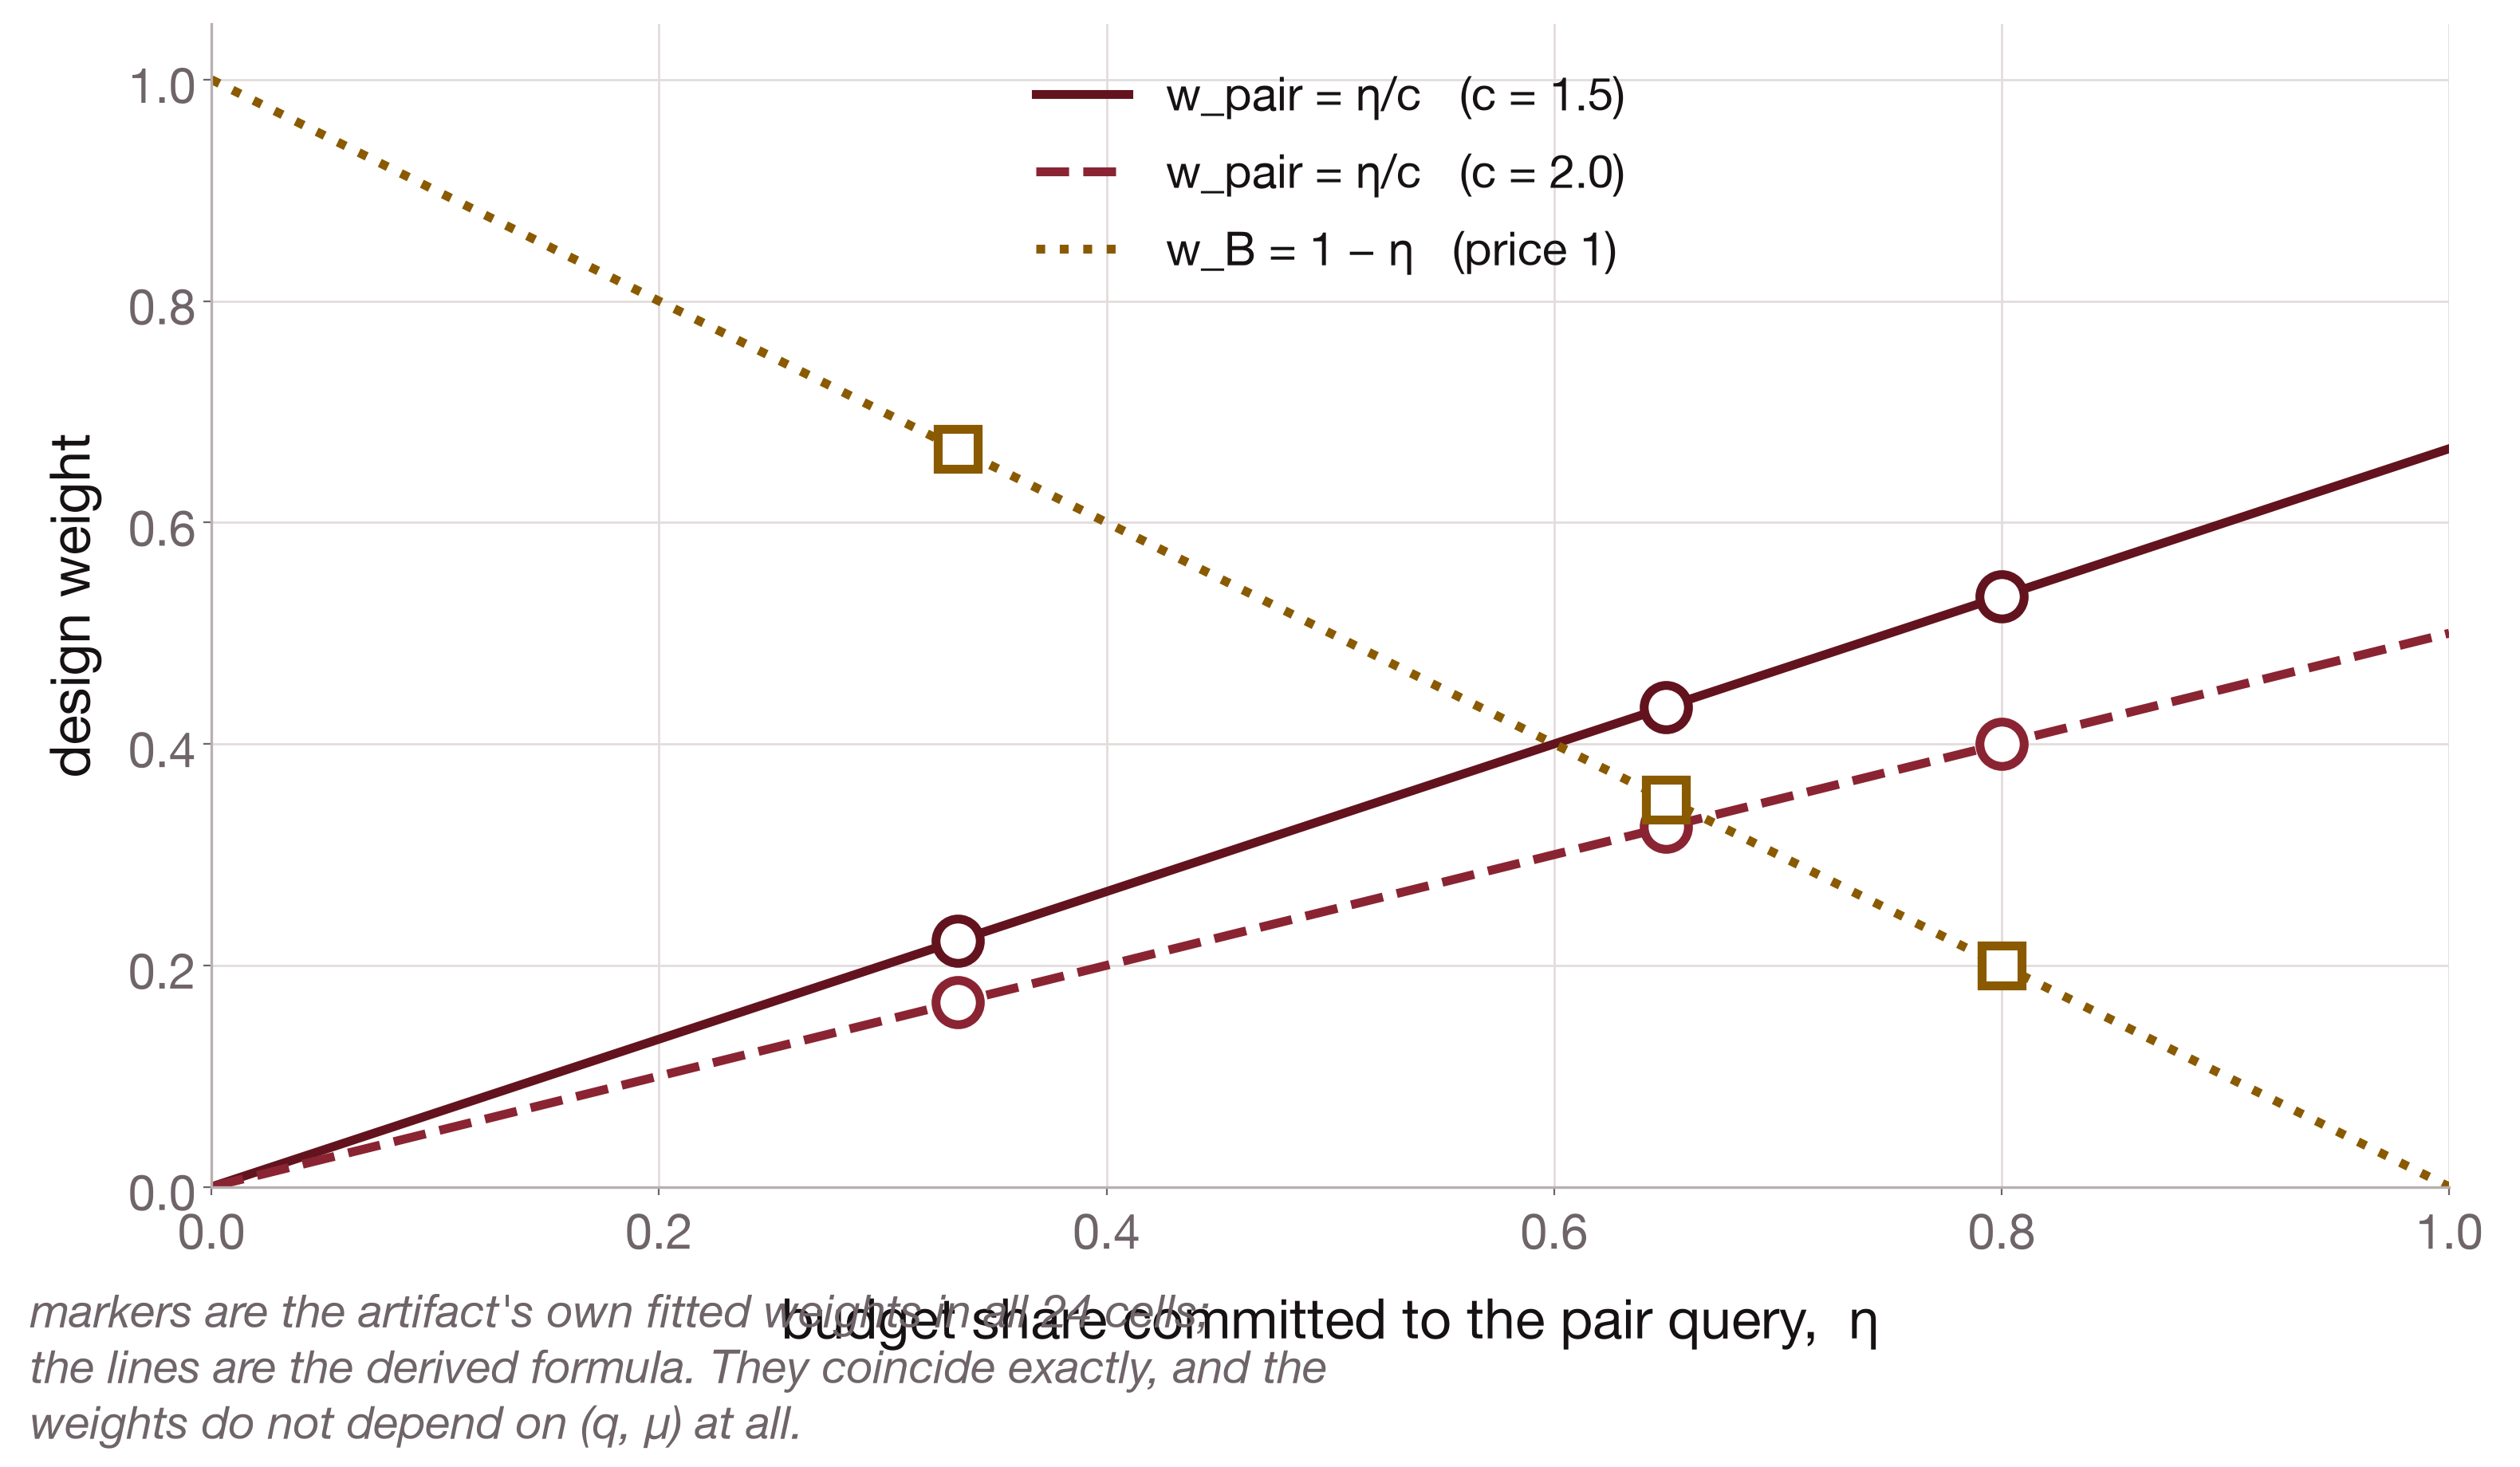
\includegraphics[width=\columnwidth]{d6_fig1_design.png}
\caption{Derived weights against the budget split. The lines are the formula
\eqref{eq:design}; the markers are the artifact's own fitted weights in all $24$ cells of
Table~\ref{tab:cells}. They coincide exactly, and---as
Corollary~\ref{cor:indep} predicts---the weights do not depend on the model parameters
$(q,\mu)$, so each marker stands for several cells that differ in $(q,\mu)$ and share
$(\eta,c)$.}
\label{fig:design}
\end{figure}

\section{A worked instance}
\label{sec:worked}

The statements are short enough that a single instance makes them concrete.

Take $q=8$, $d=3$, $\mu=\tfrac14$ and $x=\tfrac{1}{10}$. The slice information
\eqref{eq:ib} is
\begin{equation}
I_{B}(3,\tfrac{1}{10})
=\frac{1}{2}\left(\frac{3\cdot\frac{1}{16}}{8}+\frac{5\cdot\frac{1}{100}}{8}\right)
=\frac{1}{2}\cdot\frac{\frac{3}{16}+\frac{1}{20}}{8}
=\frac{19}{1280}.
\end{equation}

Now take a general alternative in the same class---say $v$ with three coordinates at
$\tfrac14,\tfrac13,\tfrac12$ (all at least $\mu$) and five at
$\tfrac{1}{10},\tfrac{1}{5},\tfrac{1}{10},\tfrac{3}{10},\tfrac{1}{10}$ (all at least $x$).
Then $\sum v_{i}^{2}=\tfrac{1}{16}+\tfrac19+\tfrac14+\tfrac{1}{100}+\tfrac{1}{25}
+\tfrac{1}{100}+\tfrac{9}{100}+\tfrac{1}{100}$, and dividing by $2q=16$ gives
$I(v)\approx 0.0345$, comfortably above $\tfrac{19}{1280}\approx 0.0148$. The excess is
exactly the sum of the coordinate-wise slacks, which is what the proof of
Theorem~\ref{thm:reduction} makes explicit.

Shrinking every coordinate to its bound recovers $I(v)=I_{B}$, which is
Corollary~\ref{cor:tight}; and any single non-zero coordinate keeps $I(v)>0$, which is
Theorem~\ref{thm:nonblind}. The three statements are visible in one instance because they
are three readings of the same sum of squares.

\subsection{Why the slice is the extreme point}

The reason the slice is cheapest has a one-line explanation that the formal proof encodes
but does not narrate. The class is defined by \emph{lower} bounds on coordinate magnitudes,
and the objective is an increasing function of each magnitude. A minimiser therefore sits
where every constraint is active, and the set of points where every constraint is active is
exactly the slice.

Put that way, the result looks inevitable, and in a sense it is---but only once the class is
described as it is here. The reason the objection had force is that the corpus described the
family constructively, as ``$d$ coordinates at $\mu$ and the rest at $x$'', which gives no
indication whether it is a restriction or an extreme point of something larger.
Theorems~\ref{thm:slice} and \ref{thm:reduction} together supply the missing description:
it is the extreme point, and the enclosing class is the one cut out by the magnitude
bounds.

\section{The separation certificate on a cell}
\label{sec:certificate}

The design results above are exact algebra. A separate question is whether a claimed strict
separation survives across a whole parameter cell rather than at the sampled points, and
that question is settled by a certificate.

\begin{theorem}[Separation across a cell]
\label{thm:modulus}
On a cell $[t_{0},t_{1}]$, if
\begin{equation}
L_{\mathrm{full}}(t_{0})\;>\;\rho_{\mathrm{two}}\;U_{\mathrm{two}}(t_{0}),
\qquad \rho\;=\;r^{(t_{1}-t_{0})/q},
\label{eq:modulus}
\end{equation}
then the strict separation holds throughout the cell.
\end{theorem}

\leanbox{\lean{quadratic\_inf\_Icc}, \lean{no\_crossing\_of\_modulus},
\lean{crossing\_bracket} in \lean{LeanD6AlternativeReductionV1}}

Two features of \eqref{eq:modulus} deserve comment. The continuous $x$-range is reduced to a
three-point check by a quadratic-infimum lemma---a quadratic on an interval attains its
infimum at an endpoint or at its vertex, so three evaluations suffice---and the modulus is
propagated across the cell by the exact multiplicative factor $\rho$. Both verdicts use
outward \emph{rational} enclosures and exact gaps rather than floating point, so a
certificate is a proof about the cell and not a statement about the sampled points in it.

\subsection{The three-point reduction}

The quadratic-infimum lemma behind Theorem~\ref{thm:modulus} is elementary and worth
stating, because it is what turns a continuum of alternatives into a finite check.

\begin{lemma}[Quadratic infimum on an interval]
\label{lem:quadinf}
For $f(x)=ax^{2}+bx+c$ with $a\ge0$ and an interval $[l,u]$,
\begin{equation}
\inf_{x\in[l,u]}f(x)\;=\;
\min\bigl\{\,f(l),\;f(u),\;f(x^{\dagger})\,\bigr\},
\end{equation}
where $x^{\dagger}=-b/2a$ when $a>0$ and $x^{\dagger}\in[l,u]$, and the third term is
omitted otherwise.
\end{lemma}

\leanbox{\lean{quadratic\_inf\_Icc} in \lean{LeanD6AlternativeReductionV1}}

The information \eqref{eq:ib} is quadratic in $x$ with non-negative leading coefficient
$(q-d)/2q$, so Lemma~\ref{lem:quadinf} applies directly: the worst alternative over a
continuous range of $x$ is found at one of three points, and the check is finite. Without it
the certificate would have to quantify over an interval, which a formal development can do
but a decision procedure cannot.

\subsection{Why rational enclosures}

The certificate \eqref{eq:modulus} compares two quantities and concludes a strict
inequality. A floating-point evaluation cannot support such a conclusion when the gap is
small, because the rounding error is unquantified relative to the gap. The development
therefore uses outward rational enclosures: each side is bracketed by exact rationals with
the bracket widened in the safe direction, and the verdict is issued only when the brackets
are disjoint.

This is what makes the eight-of-eight result in Section~\ref{sec:results} a certificate
rather than a measurement. It also explains why a cell can return \textsc{undetermined}
without the argument having failed: if the enclosures overlap, the honest output is that the
gap was not resolved at the working precision, and the remedy is a tighter enclosure rather
than a different conclusion.

\section{Results}
\label{sec:results}

\subsection{The derived weights match all 24 cells exactly}

Across $q\in\{8,16\}$, $\mu\in\{\tfrac14,\tfrac25\}$, $c\in\{\tfrac32,2\}$ and
$\eta\in\{\tfrac13,\tfrac{13}{20},\tfrac45\}$, the previously fitted weights agree with
\eqref{eq:design} in every cell, and the budget identity \eqref{eq:budget} holds exactly in
each (Table~\ref{tab:cells}). The weights vary with $(\eta,c)$ and are constant across
$(q,\mu)$, exactly as Corollary~\ref{cor:indep} predicts.

The logical status of this table changed with Section~\ref{sec:design}. Before the
derivation it was the evidence---$24$ consistent cells, suggestive but not conclusive. After
it, the table is a check on the arithmetic: the theorem says the agreement must hold at every
$(q,\mu,c,\eta)$, and the table confirms the implementation agrees with the theorem on the
cells where the fit had been performed.

\subsection{What the table looked like before and after}

It is worth being concrete about what changed, since the same $24$ numbers appear in both
accounts.

\emph{Before.} A search produced, for each cell, a pair of non-negative weights reproducing
the corpus's coefficients. The pairs were consistent: they satisfied the budget, they were
non-negative, and---noticed after the fact---they did not vary with $(q,\mu)$. The
strongest statement supportable was ``a consistent solution exists in $24$ of $24$ cells'',
which is evidence that the coefficients come from the model rather than from the search, and
nothing more. In particular it licensed no prediction at a $25$th cell.

\emph{After.} Theorem~\ref{thm:unique} says that at any $(\eta,c)$ the admissible pair is a
single point, computed by \eqref{eq:design}. The $24$ cells are then not $24$ pieces of
evidence but $24$ evaluations of one formula, and the observed independence from $(q,\mu)$
is Corollary~\ref{cor:indep} rather than a coincidence. A prediction at any further cell
follows.

The distinction is visible in what a disagreement would have meant. Before, a cell where the
fit failed would have been a puzzle to investigate. After, it would be an implementation
bug, because the theorem leaves no room for a cell to behave differently.

\subsection{The separation is certified on every cell tested}

Eight of eight cells certify the strict separation across the whole cell, all of them by the
left-endpoint test of \eqref{eq:modulus}, with exact rational gaps. That every certificate
came from the same endpoint is itself informative: the modulus decays across the cell, so
the binding case is the left edge, and a procedure that tested the midpoint would have been
testing the easy case.

\subsection{The pair query is necessary wherever it is used}

\begin{figure}[htbp]
\centering
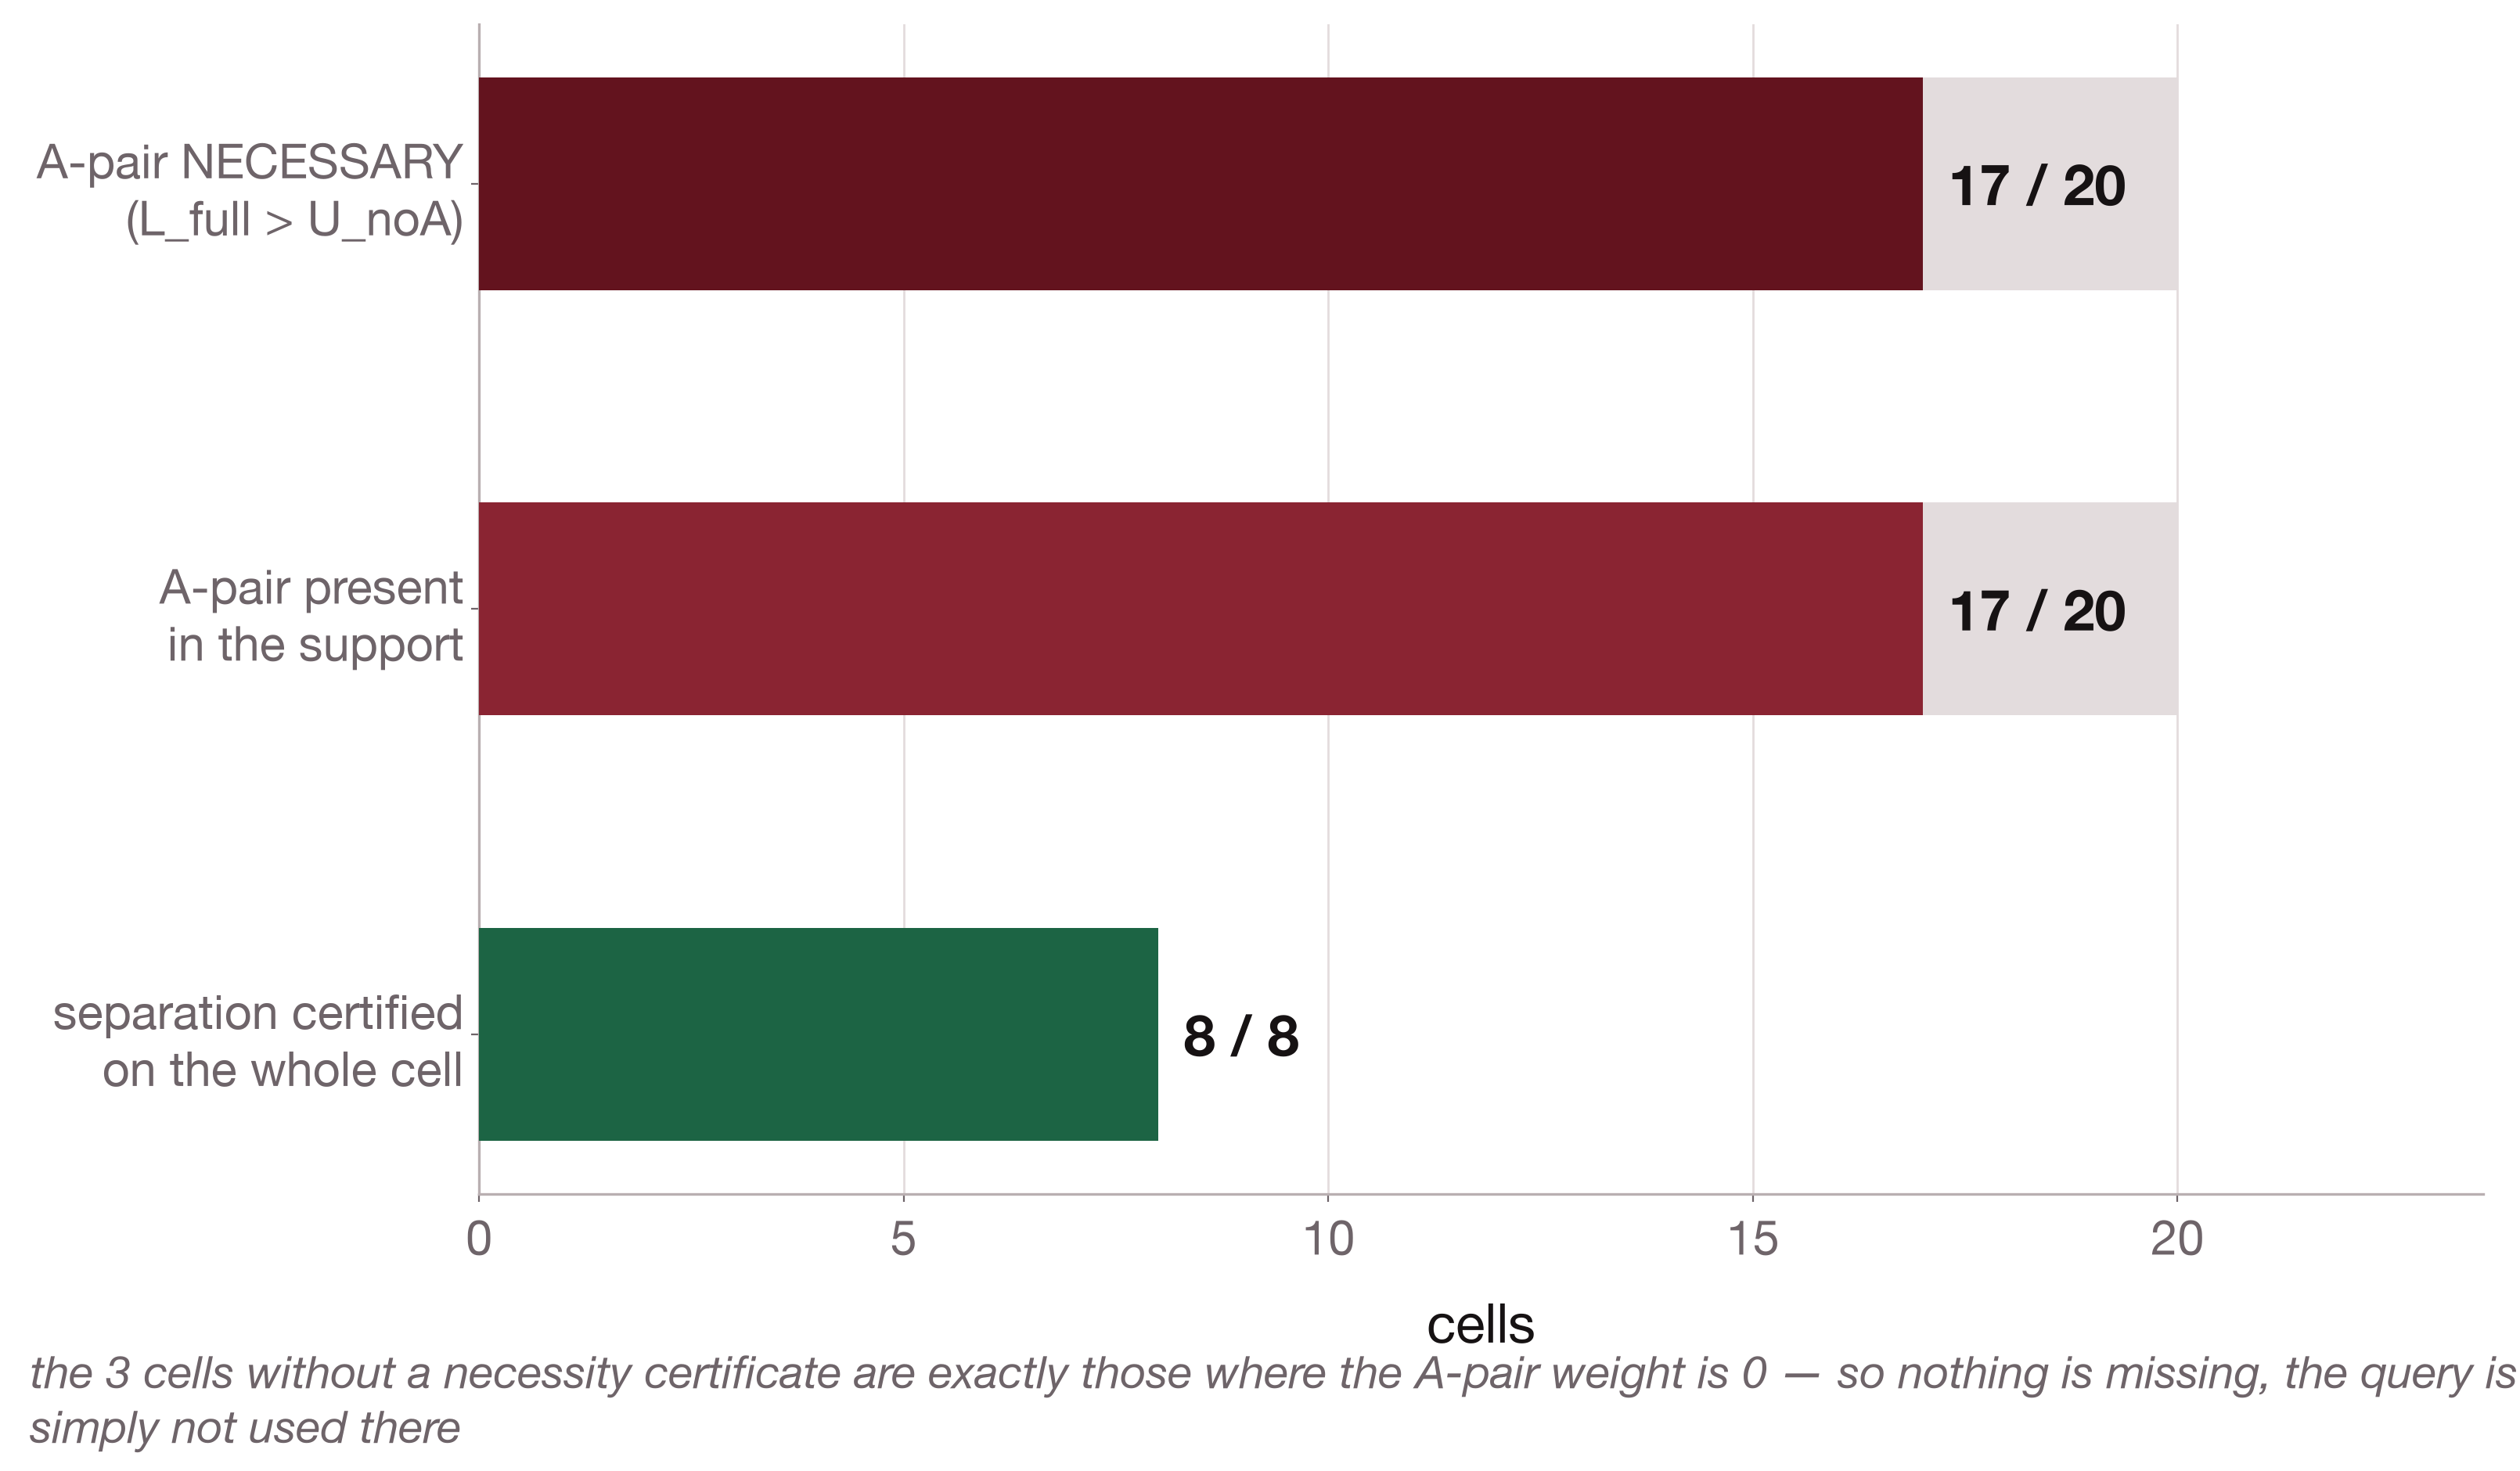
\includegraphics[width=\columnwidth]{d6_fig2_certificates.png}
\caption{Certificate counts. On $20$ parameter cells the pair query carries positive weight
in $17$, and its necessity is certified in all $17$: the full value strictly exceeds the
best achievable without it. The three cells without a certificate are exactly those where
the pair weight is zero, so nothing is missing---the query is simply not used there.}
\label{fig:certificates}
\end{figure}

On $20$ parameter cells the pair query carries positive weight in $17$, and in all $17$ its
necessity is certified: the full value strictly exceeds the best value achievable without
it. The three cells without a certificate are exactly those where the pair weight is zero.
The coincidence of those two sets is the point---a missing certificate here indicates a cell
where the query is unused, not a cell where the argument failed.

\section{The transition condition read carefully}
\label{sec:transition}

Theorem~\ref{thm:transition} says the optimum is at an endpoint unless
$c\,I_{B}=I_{\mathrm{pair}}$. The condition is simple enough to be misread in two ways, and
both readings would be wrong.

\subsection{It is not a claim that a transition occurs}

The theorem locates where a transition \emph{can} occur. Whether the condition is ever met
depends on the actual values of $I_{B}$ and $I_{\mathrm{pair}}$ at the parameters of
interest, which the theorem says nothing about. If $c\,I_{B}>I_{\mathrm{pair}}$ throughout
the parameter range, the scalar query is always the better buy, the optimum is always
$\eta=0$, and no transition exists anywhere---which is consistent with
Theorem~\ref{thm:transition} and would make a phase-boundary claim false. The paper's scope
section states this explicitly because the shape of \eqref{eq:transitioncond} invites the
stronger reading.

\subsection{It is a knife-edge, and what happens on it}

When the condition does hold, the conclusion is unusual: \emph{every} split is optimal,
because the objective \eqref{eq:affine} is constant in $\eta$. This is not a degenerate case
to be perturbed away. It says that on the knife edge the design is genuinely undetermined by
information considerations, and any choice of $\eta$ delivers the same value, so the split
may be fixed on other grounds---robustness, variance of the realised design, or
implementation convenience.

An optimiser run at such a point will return whichever $\eta$ its tie-breaking rule prefers
and report it as the optimum, which is true but uninformative. Knowing the objective is
affine lets the designer recognise the situation instead of reading a spurious structure
into the returned value.

\subsection{Why the comparison is per unit price}

The condition is $c\,I_{B}=I_{\mathrm{pair}}$ rather than $I_{B}=I_{\mathrm{pair}}$, and the
factor $c$ is the price of the pair query relative to the scalar one. Dividing through, the
condition reads
\begin{equation}
\frac{I_{B}}{1}\;=\;\frac{I_{\mathrm{pair}}}{c},
\end{equation}
i.e.\ the two queries deliver equal information per unit of budget spent. That is the form
worth remembering, and it is what makes the threshold interpretable: the design is pure
toward whichever query offers more information per unit price, and mixed only when neither
does.

\section{Threats to the argument}
\label{sec:threats}

Three ways the results could fail to mean what they appear to, with what rules each out.

\emph{The class could be the wrong class.} Theorem~\ref{thm:reduction} quantifies over
alternatives satisfying per-coordinate magnitude bounds. If the alternatives that actually
threaten a decision do not satisfy those bounds---if some coordinate may be left
undisplaced---the reduction covers a set that does not contain them, and the upgrade is
vacuous for the purpose. Nothing in the formal development can detect this, because it is a
modelling question; what the development does is make the hypothesis explicit in the
statement, so the mismatch is visible to a reader rather than buried in a derivation.

\emph{The information formulas could be wrong.} $I_{B}$ and $I_{\mathrm{pair}}$ are taken
from the corpus and not re-derived from the sampling model. If either is mis-stated, every
downstream conclusion inherits the error, including the transition condition
\eqref{eq:transitioncond}, which compares them directly. This is a genuine dependency and is
listed in the scope section for that reason. It is also the dependency most easily audited,
since the formulas are two lines each.

\emph{The split could not be the right parameterisation.} Theorem~\ref{thm:unique} takes the
split $\eta$---the budget share committed to the pair query---as given, and derives the
weights from it together with the budget. A different parameterisation of the same feasible
segment would give different-looking weights satisfying the same budget, and someone
comparing the two could conclude the derivation is not unique. It is: the segment is
one-dimensional and \eqref{eq:design} parameterises it by $\eta$; a reparameterisation is a
change of coordinate on the same set, not a different design. The formal statement fixes the
coordinate by taking $c\,w_{\mathrm{pair}}=\eta$ as a hypothesis, which is where the
convention is recorded.

None of the three is resolved by computation, and all three are stated so that a reader can
check them against their own setting rather than accept them.

\section{Formal verification}
\label{sec:verification}

Every theorem above is machine-checked in Lean~4, toolchain
\texttt{leanprover/lean4:v4.34.0-rc2} against mathlib revision \texttt{1f495c61}.

\subsection{Acceptance contract}

A module counts as accepted only when all six of the following hold: the compiler exits zero
with no errors; the source hash is unchanged \emph{across} the compile; the compiled
artifact is newer than its source; at least one \texttt{\#print axioms} directive is
present; the axiom set of every audited declaration lies within
$\{\textsf{propext},\textsf{Classical.choice},\textsf{Quot.sound}\}$; and no \texttt{sorry}
appears anywhere in the file.

\subsection{The crux statements as they are checked}

\begin{figure}[htbp]
\footnotesize
\hrule\vspace{4pt}
\begin{tabbing}
\quad\=\quad\=\kill
\lean{theorem IB\_le\_general (q : $\mathbb{N}$) (hq : 0 < q)} \\
\> \lean{(mu x : $\mathbb{Q}$) (hmu : 0 $\le$ mu) (hx : 0 $\le$ x)} \\
\> \lean{(v : Fin q $\to$ $\mathbb{Q}$) (S : Finset (Fin q))} \\
\> \lean{(hS : $\forall$ i $\in$ S, mu $\le$ |v i|)} \\
\> \lean{(hSc : $\forall$ i, i $\notin$ S $\to$ x $\le$ |v i|) :} \\
\> \lean{IB (q : $\mathbb{Q}$) (S.card : $\mathbb{Q}$) mu x $\le$ Igen q v} \\[6pt]
\lean{theorem weights\_unique (eta c a b : $\mathbb{Q}$) (hc : c $\ne$ 0)} \\
\> \lean{(hbudget : a + c * b = 1) (hshare : c * b = eta) :} \\
\> \lean{a = wB eta $\wedge$ b = wPair eta c}
\end{tabbing}
\vspace{-4pt}\hrule
\caption{The reduction and the uniqueness, as checked. Both are over $\mathbb{Q}$, so every
arithmetic step is exact. In \lean{IB\_le\_general} the shift \lean{v} is an arbitrary
function \lean{Fin q $\to$ $\mathbb{Q}$} and the block \lean{S} an arbitrary \lean{Finset};
the hypotheses are the per-coordinate magnitude bounds and nothing else, so the conclusion
holds for every alternative in the class rather than for a parameterised family. In
\lean{weights\_unique} the conclusion is an equality, not an existence, which is what
distinguishes a derivation from a fit---and the hypothesis is \lean{c $\ne$ 0}, with
positivity of the price entering separately through
\lean{weights\_nonneg\_iff}.}
\label{fig:statements}
\end{figure}

The quantifier structure of \lean{IB\_le\_general} is the whole content of C1. The shift
vector is an arbitrary function and the displaced block an arbitrary finite set; nothing in
the statement mentions a two-parameter family, and the two-parameter formula appears only on
the left of the inequality as the quantity being bounded below. A statement that instead
quantified over $(d,x)$ and concluded something about $(d,x)$ would be the original result,
not an upgrade of it.

Likewise \lean{weights\_unique} concludes an \emph{equality} from the budget and the split.
An existential---``there exist non-negative weights satisfying the budget''---would be
consistent with the weights having been fitted; the equality is what rules that out.

\subsection{What the paper derives rather than cites}

Two displayed corollaries carry no \lean{leanbox} because the paper obtains them from the
checked statements: Corollary~\ref{cor:upgrade}, which chains
Theorem~\ref{thm:reduction} with a hypothesis on $I_{B}$, and
Corollary~\ref{cor:indep}, which reads off \eqref{eq:design} that $q$ and $\mu$ do not
occur. Both are immediate, and both are named here so that the reader is not left to infer
which results are checked and which are consequences drawn in the text.

\subsection{Evidence per step}

\begin{table}[htbp]
\caption{Evidence per step. All cited declarations are axiom-audited.}
\label{tab:inventory}
\centering
\footnotesize
\setlength{\tabcolsep}{3pt}
\begin{tabular}{@{}llr@{}}
\toprule
Step & Module & Aud. \\
\midrule
Slice identity, Thm~\ref{thm:slice}    & \lean{LeanD6GeneralFamilyV1}       & 5 \\
Reduction, Thm~\ref{thm:reduction}     & \lean{LeanD6GeneralFamilyV1}       & 5 \\
Tightness, Cor~\ref{cor:tight}         & \lean{LeanD6GeneralFamilyV1}       & 5 \\
Positivity, Thm~\ref{thm:nonblind}     & \lean{LeanD6GeneralFamilyV1}       & 5 \\
Budget, Thms~\ref{thm:budget}--\ref{thm:unique} & \lean{LeanD6DesignDerivationV1} & 7 \\
Affine, Thm~\ref{thm:affine}           & \lean{LeanD6DesignDerivationV1}    & 7 \\
Transition, Thm~\ref{thm:transition}   & \lean{LeanD6DesignDerivationV1}    & 7 \\
Separation, Thm~\ref{thm:modulus}      & \lean{LeanD6AlternativeReductionV1}& 7 \\
\bottomrule
\end{tabular}
\end{table}

\subsection{Why a large strand yields few displayed equations}

The D6 strand is by far the largest in the programme---$444$ files and $4{,}087$ statements
against, for instance, the Query strand's $21$ and $135$---and it contributes five displayed
equations to this paper. The ratio invites the question of what the rest is doing, and the
answer is worth giving because it is characteristic of formal developments and misleading if
left implicit.

Most of the strand is search and refutation. Establishing that the $(d,x)$ family is the
right one required first establishing that several other candidate families were not: each
withdrawn formulation leaves behind the statements that ruled it out, and those statements
are correct, checked, and not displayed because they support a claim the paper does not
make. Similarly, the separation certificates of Section~\ref{sec:certificate} are issued per
cell, so the file count scales with the parameter grid rather than with the mathematical
content.

What is displayed is the shortest path from the two objections to their answers. A reader
auditing the claim needs the eight declarations of Table~\ref{tab:inventory}; a reader
auditing the \emph{programme} would need the rest, and would find in it mostly a record of
what did not work.

\subsection{Scope of the formalisation}

The displayed results are the load-bearing chain, not the corpus. The D6 strand contains
$444$ Lean source files with $4{,}087$ theorem and lemma statements, of which $28$ modules
carry an acceptance receipt covering $175$ declarations whose axiom set was printed and
checked. Across the programme of which this paper is one part: $762$ files, $7{,}199$
statements, $108$ accepted modules, $860$ audited declarations.

No module cited in this paper contains a \texttt{sorry}. Seven occurrences exist in the
wider repository, in audit scaffolding and in files named as conjectures; the overlap
between the cited set and the files containing them was computed and is empty.

\section{Generalising the two arguments}
\label{sec:general}

Neither argument is specific to this query pair, and saying which features they need makes
clear where else they apply.

\subsection{When does a family become extremal?}

Theorem~\ref{thm:reduction} needs two things: the class must be cut out by \emph{lower}
bounds on per-coordinate quantities, and the objective must be increasing in each of those
quantities. Given both, the minimiser is where every constraint is active, and if that set
is the family in question then the family is extremal.

The recipe therefore transfers to any information functional that is a sum of increasing
per-coordinate terms---which covers the quadratic form here, and also any $\sum_{i}\phi(v_i)$
with $\phi$ even and increasing on $[0,\infty)$. It fails as soon as the objective has a
cross term, because then reducing one coordinate to its bound can increase the objective
through another, and the active set need not be the minimiser. This is precisely why the
pair query is not covered: its information is not separable across coordinates.

\subsection{When is a design forced?}

Theorem~\ref{thm:unique} needs the feasible set to be a segment---one budget equation, two
weights---and the parameterisation to be fixed by a second linear condition. With three query
types the feasible set is a two-dimensional simplex slice, one budget equation no longer
determines the design given a scalar split, and the uniqueness fails. What survives is that
the objective remains linear in the weights, so the optimum is still at a vertex; what is
lost is that the vertex is no longer one of two, and the comparison
\eqref{eq:transitioncond} becomes a comparison among several information-per-price ratios.

That generalisation looks routine and is listed as an open problem rather than asserted,
because the admissible range of the multi-dimensional split---the analogue of
Proposition~\ref{prop:nonneg}---is a polytope rather than an interval, and whether it is
cut out as cleanly is not obvious from the two-query case.

\section{Discussion}
\label{sec:discussion}

\subsection{Why the two halves belong in one paper}

The reduction and the design derivation answer different objections and use different
techniques, and a reader may reasonably ask why they appear together. The reason is that
each is incomplete without the other for the purpose either serves.

The reduction upgrades a lower bound on $I_{B}$ to a lower bound over the class. That upgrade
is useful only if $I_{B}$ is the quantity a design actually delivers, which is what
Section~\ref{sec:design} establishes: the delivered information at split $\eta$ is
\eqref{eq:affine}, a combination of $I_{B}$ and $I_{\mathrm{pair}}$ with weights that are
forced rather than chosen. Without the design derivation, the reduction would be a statement
about a quantity whose relationship to any implementable design was unsettled.

Conversely the design derivation identifies the optimal split by comparing $c\,I_{B}$ with
$I_{\mathrm{pair}}$. That comparison is meaningful only if $I_{B}$ is what the scalar query
is worth against the alternatives that matter---which is exactly what the reduction
establishes. Without it, the comparison would be between the pair query's value against its
class and the scalar query's value against a slice.

\subsection{Two objections of different kinds}

C1 is a statement about \emph{quantifiers}: it converts a slice-quantified lower bound into
a class-quantified one, and it is the reason the two-parameter family may now be used
without apology. C4 is a statement about \emph{provenance}: it replaces a fit with a
derivation, so the weights are no longer numbers that happened to work in the cells tested.

The distinction matters for how each should be judged. A quantifier error is repaired by an
argument or not at all---no quantity of additional alternatives sampled from outside the
slice would establish Theorem~\ref{thm:reduction}, because the claim is universal. A
provenance gap is likewise not closed by more cells; the $24$ cells were already consistent,
and the missing ingredient was a reason.

\subsection{The practical payoff}

C5 is where C4 pays. Once the design is a function of $(\eta,c)$, the delivered information
becomes affine in the split, and an affine objective has no interior optimum. The design is
therefore pure on either side of the explicitly computable threshold
\eqref{eq:transitioncond}, and that threshold is derived from the model rather than
declared. A designer does not need to search over $\eta$; they need to compare $c\,I_{B}$
against $I_{\mathrm{pair}}$ and commit the whole budget accordingly.

\subsection{On the value of negative-sounding results}

Three of this paper's statements sound like limitations and are in fact the contribution.
Corollary~\ref{cor:tight} says the bound cannot be improved by enlarging the class---which
reads as a ceiling, but is what makes the reduction free. Theorem~\ref{thm:unique} says
there is no freedom in the weights---which reads as a loss of generality, but is what
converts a fit into a derivation. Theorem~\ref{thm:transition} says the optimum is at an
endpoint---which reads as a degenerate answer, but is what removes the need to search.

The pattern is common enough to name. A result that closes off possibilities is worth as
much as one that opens them, provided the closure is proved rather than observed, because it
tells a designer where not to spend effort. Here the three closures together mean that a
reader with $(\eta,c)$ in hand does no optimisation at all: the weights are given by a
formula, the split is an endpoint, and the bound they are working against covers every
alternative in the class.

\subsection{What is not established}

\begin{enumerate}
\item \textbf{The reduction is for the scalar query.} The pair query has a blind direction
and is not covered by Theorem~\ref{thm:reduction}. Nothing here upgrades a slice bound for
that query.

\item \textbf{Lower bounds only.} As noted after Corollary~\ref{cor:upgrade}, an upper bound
quantified over the slice still says nothing about the class.

\item \textbf{The class is cut out by magnitude constraints.} An alternative set defined
otherwise---by a norm bound, say, or by a linear subspace---is outside the statement.

\item \textbf{The information formulas are taken as given.} They are not re-derived from the
sampling model, so a reader who disputes them disputes the premises rather than the
argument.

\item \textbf{The uncapped profile.} The design derivation is for the uncapped profile;
where the unconstrained nuisance minimiser leaves its window, the clipped branch applies and
is settled separately.

\item \textbf{No phase boundary is proved.} Theorem~\ref{thm:transition} identifies where a
transition \emph{can} occur. It does not establish that the condition is met anywhere in the
parameter range of interest, and no phase diagram is claimed.
\end{enumerate}

\subsection{What formalisation caught}

Two formulations were withdrawn under the prover.

The first attempt at Theorem~\ref{thm:reduction} stated the hypothesis as
$v_{i}\ge\mu$ rather than $|v_{i}|\ge\mu$. The conclusion is still true under that stronger
hypothesis, but the class it describes is one-sided---it excludes alternatives displacing a
coordinate downward---and the reduction would then have upgraded a slice bound only to a
half-space, which is not what C1 claims. Restoring the absolute values made the class
symmetric and cost nothing in the proof, since the argument uses $|v_{i}|^{2}=v_{i}^{2}$
either way.

The second was in the budget derivation. An early version of Theorem~\ref{thm:budget}
omitted the hypothesis $c>0$ and was accepted for the identity \eqref{eq:budget}, which is
indeed true for any $c\neq0$. But \lean{weights\_nonneg\_iff}---
Proposition~\ref{prop:nonneg}---then failed, because with $c<0$ the weight
$w_{\mathrm{pair}}=\eta/c$ is non-positive on the whole admissible range of $\eta$. The
hypothesis was added where it belongs, and the admissible range became a derived statement
rather than an assumed one.

Neither error changes a number. Both change what the statements mean, which is the category
of defect this paper exists to remove.

\subsection{How to use these results}

For a reader who wants to apply rather than audit, the three usable statements are these.

\emph{Use the slice bound without apology.} If a lower bound $L$ has been proved by
quantifying over $(d,x)$, Corollary~\ref{cor:upgrade} makes it a lower bound over every
alternative in the magnitude-constrained class. Check only that the class is the one cut out
by per-coordinate magnitude bounds, since that is the hypothesis
Theorem~\ref{thm:reduction} uses.

\emph{Compute the design, do not search for it.} Given the price $c$ and the split $\eta$,
the weights are \eqref{eq:design} and nothing else; by Theorem~\ref{thm:unique} there is no
other admissible pair, so a search over designs at fixed $(\eta,c)$ has a one-point feasible
set. Do check $0\le\eta\le1$ and $c>0$, which by Proposition~\ref{prop:nonneg} is exactly
the condition for both weights to be non-negative.

\emph{Do not search over the split either.} By Theorem~\ref{thm:transition} the delivered
information is affine in $\eta$, so the optimum is at an endpoint. Compare $c\,I_{B}$ with
$I_{\mathrm{pair}}$: if the former is smaller, commit the budget to the pair query; if
larger, to the scalar query; if equal, every split is optimal and the choice may be made on
other grounds.

The third item is the one most likely to save work in practice, because a designer who does
not know the objective is affine will naturally grid-search $\eta$ and report an interior
optimum produced by numerical noise.

\subsection{Open problems}

Whether the reduction extends to the pair query, in some form that accounts for its blind
direction, is the natural next question; the obstruction is that
Theorem~\ref{thm:reduction}'s coordinate-wise argument needs every coordinate to contribute,
which the pair query's kernel prevents. Whether the affine structure of
Theorem~\ref{thm:affine} survives three or more query types---where the budget simplex is no
longer an interval and an interior optimum becomes possible---is the second. And whether
condition \eqref{eq:transitioncond} is ever met on the parameter range of interest, which
would turn Theorem~\ref{thm:transition} from a possibility statement into a phase boundary,
is the third.

\section{Conclusion}

The two-parameter alternative family is not a restriction: every alternative in its class
costs at least the slice value, and the bound is attained exactly on the slice. The design
that reproduces the corpus's coefficients is not fitted: it is forced by the budget
constraint and the split, depends only on the split and the price, and makes the delivered
information affine---so the optimal design is pure except on an explicitly computable
threshold.

The wider point is about how a corpus of results should be maintained. Both objections
answered here were raised against statements that were, numerically, entirely correct: the
slice bounds hold, and the fitted weights are the right weights. What was missing in each
case was an argument connecting the statement to the claim it was being used to support, and
in both cases the missing argument turned out to be short. Finding that a gap is small is
not the same as finding that it is absent, and the difference is only visible once someone
tries to write the connecting step down.

\section*{Acknowledgment}

The formal development uses the Lean~4 theorem prover and the mathlib library.

\begin{thebibliography}{00}

\bibitem{pukelsheim2006} F. Pukelsheim, \emph{Optimal Design of Experiments}. Philadelphia,
PA: SIAM Classics in Applied Mathematics, 2006.

\bibitem{boyd2004} S. Boyd and L. Vandenberghe, \emph{Convex Optimization}. Cambridge,
U.K.: Cambridge Univ. Press, 2004.

\bibitem{mathlib2020} The mathlib Community, ``The Lean mathematical library,'' in
\emph{Proc. 9th ACM SIGPLAN Int. Conf. Certified Programs and Proofs (CPP)}, 2020,
pp.~367--381.

\bibitem{demoura2021} L. de Moura and S. Ullrich, ``The Lean 4 theorem prover and
programming language,'' in \emph{Proc. 28th Int. Conf. Automated Deduction (CADE)}, 2021,
pp.~625--635.

\bibitem{fedorov1972} V. V. Fedorov, \emph{Theory of Optimal Experiments}. New York, NY:
Academic Press, 1972.

\bibitem{moore2009} R. E. Moore, R. B. Kearfott, and M. J. Cloud, \emph{Introduction to
Interval Analysis}. Philadelphia, PA: SIAM, 2009.

\end{thebibliography}

\end{document}
